\subsection{Share of Detected Cases}
\label{subsec:results_share_known_cases}

\begin{figure}[ht]
  \centering
  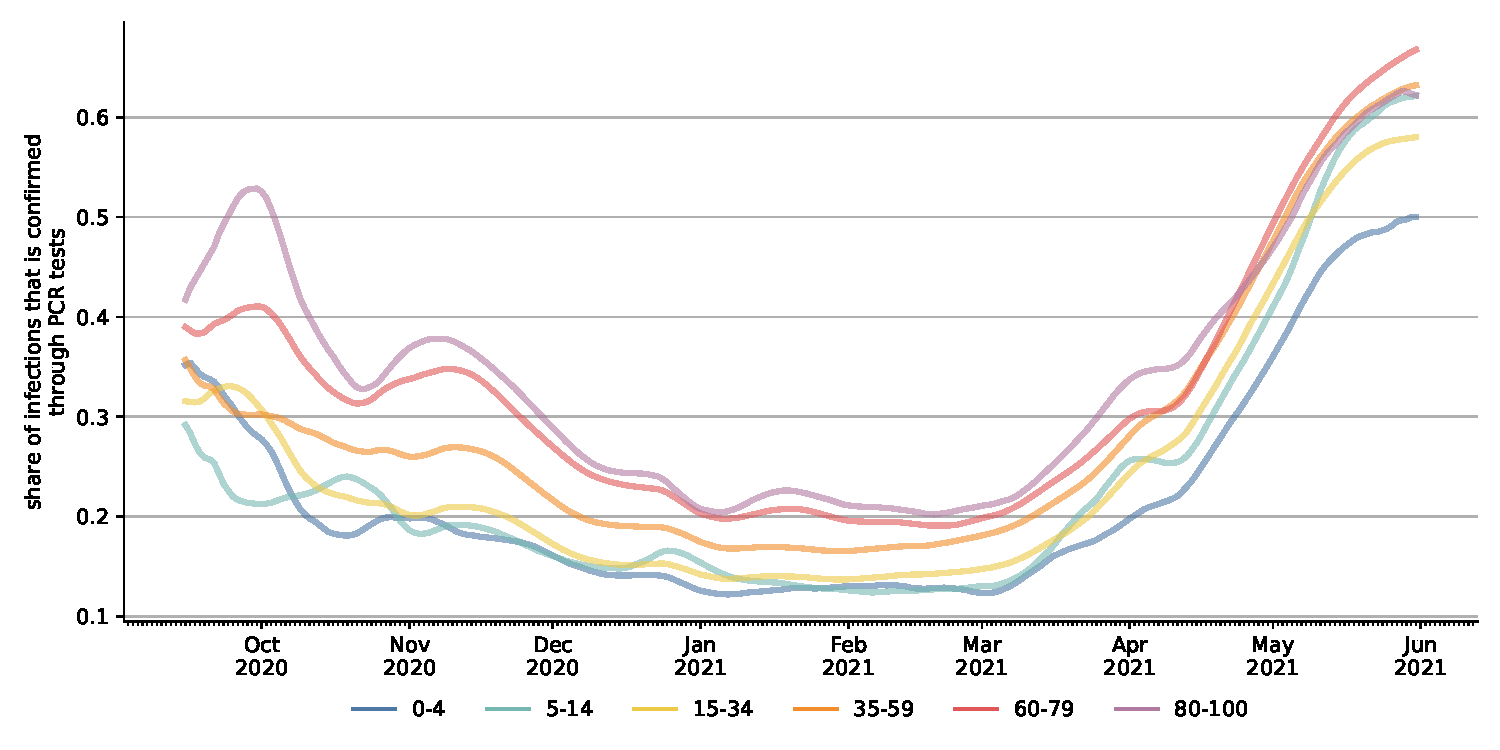
\includegraphics[width=\textwidth]{figures/results/figures/share_known_cases/full_combined_baseline_by_age_group_rki}
  \caption{Share of Detected Cases by Age Group}
  \label{fig:share_known_cases_by_age_group}
  \floatfoot{\noindent \textit{Note:} The figure shows the share of cases that is
  reported as an official case via PCR confirmation. We use the overall share of known
  cases that was estimated through the case fatality ratio by the
  \href{https://covid19.dunkelzifferradar.de/}{Dunkelzifferradar} for all of 2020 and
  then assume it to be constant as vaccinations of the elderly strongly affect the case
  fatality rate which the project does not account for. To get from an overall share of
  detected cases to the share of cases that is detected in each age group we use that
  asymptomatic cases are much less likely to be detected. As our model covers age
  specific asymptomatic rates this endogenously leads to group specific share known cases
  that verify that infections in younger age groups are under-detected. Starting in 2021
  in addition to the overall numbers of detected cases through symptoms and the share
  known cases, cases are also detected through confirmation of positive rapid tests. This
  leads to an increase in the share of known cases for all age groups but in particular
  for the younger age groups that are covered extensively with rapid tests through the
  rapid test requirement for participating in school.}
\end{figure}

It's noteworthy that the share of detected cases increases rapidly in May for the five to
fourteen year olds. This is a direct result of the mandatory tests in school.

\FloatBarrier